\documentclass[a4paper]{article}
\usepackage[left=3cm,right=3cm,top=2cm,bottom=2cm]{geometry} % page settings
\usepackage{enumerate}
\usepackage{hyperref}
\usepackage{graphicx}
\usepackage{amsfonts}
\usepackage{amsthm}
\usepackage{mathtools}
\usepackage{titlesec}
\usepackage{polski}
\usepackage{tikz}
\usepackage[utf8]{inputenc}
\DeclarePairedDelimiter\ceil{\lceil}{\rceil}
\DeclarePairedDelimiter\floor{\lfloor}{\rfloor}

\def\checkmark{\tikz\fill[scale=0.3](0,.35) -- (.25,0) -- (1,.7) -- (.25,.15) -- cycle;} 
\newcommand{\Bernstein}{$$B_{i}^{n}(u) = {n \choose i}u^i (1-u)^{n-i}$$}

\titlespacing*{\subsection}
{0ex}{10ex}{3ex}

\title{Lista 9}
\author{Kamil Matuszewski}
\date{13 grudnia 2015}

\begin{document}

\maketitle
\setlength{\parindent}{0.5ex}
\setlength{\parskip}{1.5ex}

\begin{center}
\begin{tabular}{|c *{8}{|c} |c|}\hline
1 & 2 & 3 & 4 & 5 & 6 & 7 & 8\\
\hline 
\checkmark & \checkmark & \checkmark & \checkmark & \checkmark & \checkmark & \checkmark &  \\
\hline
\end{tabular}\\
\end{center}


\subsection*{Zadanie 1}

(a) Trywialne, Spójrzmy na wzór \Bernstein Wprost z definicji wynika, że $0$ jest $i$-krotnym zerem funkcji ($u^i$), a $1$ jest $(n-i)$-krotnym zerem funkcji $\left((1-u)^{n-i}\right)$

(b) To, że $B_i^n$ jest dodatnie na przedziale $(0,1)$ wynika wprost z tego, że ma miejsca zerowe w $0$ i $1$.
$$ \begin{matrix}
u^i(1-u)^{n-i} > 0 & & & & u\in (0,1)
\end{matrix} $$ 
Dodatkowo ${n \choose i}$ jest dodatnie z definicji(można też pokazać to, że jest dodatnie indukcyjnie, korzystając ze wzoru rekurencyjnego z zadania 3)\\
Teraz, można łatwo pokazać, że pochodną wzoru \Bernstein
Jest\\
$$ {n \choose i}\left( i u^{i-1} (1-u)^{n-i} - u^i (n-i)(1-u)^{n-i-1} \right) $$
Skoro tak, to maksimum funkcji będzie:
\large
$$
\begin{matrix*}[l] 
{n \choose i}\left( i u^{i-1} (1-u)^{n-i} - u^i (n-i)(1-u)^{n-i-1} \right) = 0 &&&&& \backslash :{n\choose i} \\
i u^{i-1} (1-u)^{n-i} - u^i (n-i)(1-u)^{n-i-1} = 0 &&&&& \backslash :u^{i-1} \\
i (1-u)^{n-i} - u (n-i)(1-u)^{n-i-1} = 0 &&&&& \backslash :(1-u)^{n-i-1} \\
i (1-u) - u (n-i) = 0 \\
i-ui-(un-ui)=0 \\
i-un=0 \\
i=un &&&&& \backslash :n \\
u=\frac{i}{n}
\end{matrix*}$$
\normalsize
Warto zauważyć, że działania te możemy wykonywać tylko dlatego, że wiemy, że $u\neq 0$ oraz $u \neq 1$. Stąd nasza funkcja ma dokładnie jedno ekstremum, w punkcie $u=\frac{i}{n}$

\clearpage

\subsection*{Zadanie 2}
Wiemy, że:
$$ {n \choose k}{n-k \choose i-k} = {n \choose i}{i \choose k} $$
Najpierw, rozpiszmy $B_k^n$
$$B_k^n(t) = {n \choose k}t^k(1-t)^{n-k} = {n \choose k}t^k\sum\limits_{i=0}^{n-k}(-1)^i{n-k \choose i}t^i = \sum\limits_{i=0}^{n-k} (-1)^i {n \choose k} {n-k \choose i}t^{i+k} = \sum\limits_{i=k}^{n} (-1)^{i-k} {n \choose k} {n-k \choose i-k}t^{i}$$ 
$$= \sum\limits_{i=k}^{n} (-1)^{i-k} {n \choose i}{i \choose k} t^i$$

Teraz, pokażmy liniową niezależność:

$$0=c_0B_0^n(t) + c_1B_1^n(t) + \dots + c_nB_n^n(t)$$ 
$$= c_0 \sum\limits_{i=0}^{n} (-1)^{i} {n \choose i}{i \choose 0} t^i + c_1 \sum\limits_{i=1}^{n} (-1)^{i-1} {n \choose i}{i \choose 1} t^i + \dots + c_n \sum\limits_{i=n}^{n} (-1)^{i-n} {n \choose i}{i \choose n} t^i$$

Teraz, możemy zapisać, że(nie interesuje nas $(-1)^x$, później pokażę czemu):
$$c_0 t^0 + \left[\sum\limits_{i=0}^{1}c_i{n \choose 1}{1 \choose i} \right]t^1 + \cdots + \left[\sum\limits_{i=0}^{n}c_i{n \choose n}{n \choose i} \right]t^n$$

$t^0\dots t^n$ są liniowo niezależne, czyli dla dowolnych b $$b_0+b_1t^1 + \dots + b_nt^n = 0 \Leftrightarrow b_0=\dots=b_n=0$$ Nasze współczynniki to: $\sum\limits_{i=0}^{k}c_i{n \choose k}{k \choose i}$, stąd możemy zapisać równania:

$$
\begin{matrix*}[r]
c_0 =& 0\\ \\ 
\sum\limits_{i=0}^{1}c_i {n \choose 1}{1 \choose i} =& 0
\\ \\
\vdots
\\ \\
\sum\limits_{i=0}^{n}c_i {n \choose n}{n \choose i} =& 0

\end{matrix*}
$$

Widać, że $c_0=0$. Teraz, odejmujemy (lub dodajemy, dlatego nie obchodzi nas minus) stronami równania, tak, by w każdej kolejnej sumie zostawić tylko ostatni wyraz, np:\\

$$
\begin{matrix*}[r]
c_0 =& 0\\ \\ 
\sum\limits_{i=0}^{1}c_i {n \choose 1}{1 \choose i} =& 0 &&&& \backslash -c_0{0 \choose 1}{1 \choose 0}
\\ \\ 
c_1 {n \choose 1}{1 \choose 1} =& 0 &\Leftrightarrow c_1=0
\\ \\
\sum\limits_{i=0}^{2}c_i {n \choose 2}{2 \choose i} =& 0 &&&& \backslash -c_1{n \choose 2}{2 \choose 1} - c_0{0 \choose 2}{2 \choose 0}
\\ \\
c_2 {n \choose 2}{2 \choose 2} =& 0 &\Leftrightarrow c_2=0

\end{matrix*}
$$
Symbol newtona jest liczbą całkowitą (dodatnią), dlatego obliczając ten układ równań, wychodzi nam, że:
$$0=c_0=c_1= \dots =c_n$$
A to oznacza, że $B_0^n \dots B_n^n$ są liniowo niezależne, a jest ich $n+1$, więc jest to baza $\prod_n$
\subsection*{Zadanie 3}
(a) Wychodząc z lewej dojdę do prawej:\\
$$
(1-u)B_{n-1}^{i}(u)+uB_{n-1}^{i-1}(u) = (1-u){n-1 \choose i}u^i(1-u)^{n-1-i} + u{n-1 \choose i-1}u^{i-1}(1-u)^{n-1-(i-1)}=$$
$$={n-1 \choose i}u^i(1-u)^{n-i} + {n-1 \choose i-1}u^{i}(1-u)^{n-i}=\left[ {n-1 \choose i} + {n-1 \choose i-1} \right]u^i(1-u)^{n-i}={n \choose i}u^i (1-u)^{n-i}=B_{n}^{i}(t)$$

(b) Wykorzystamy fakt, że $B_{n}^{i}(u)=(1-u)B_{n}^{i}(u) + uB_{n}^{i}(u)$:

\large
$$ 
\begin{matrix*}[l] 
(1-u)B_{n}^{i}(u) & ={n \choose i}u^i (1-u)^{n+1-i}\\
 & = \frac{{n \choose i}}{{n+1 \choose i}} {n+1 \choose i} u^i (1-u)^{n+1-i}\\
 & = \frac{n-i+1}{n+1} B_{i}^{n+1}(u) 
\end{matrix*}
$$


$$
\begin{matrix*}[l] 
uB_{n}^{i}(u) & = {n \choose i} u^{i+1} (1-u)^{n-i}\\
& = {n \choose i} u^{i+1} (1-u)^{n+1-(i+1)} \\
& = \frac{{n \choose i}}{{n+1 \choose i+1}} {n+1 \choose i+1} u^{i+1} (1-u)^{n+1-(i+1)}\\
& = \frac{i+1}{n+1}B_{i+1}^{n+1}(u)
\end{matrix*}
$$
\normalsize

Stąd $$B_{n}^{i}(u)=(1-u)B_{n}^{i}(u) + uB_{n}^{i}(u) = \frac{n-i+1}{n+1} B_{i}^{n+1}(u) + \frac{i+1}{n+1}B_{i+1}^{n+1}(u)$$

\subsection*{Zadanie 4}
(a)
$$\sum\limits_{i=0}^{n} B_{i}^{n}(t) \equiv 1$$
$$\sum\limits_{i=0}^{n} B_{i}^{n}(t) =\sum\limits_{i=0}^{n} {n \choose i}t^i (1-t)^{n-i} \stackrel{*}{=} ((1-t)+t)^n = 1^n = 1$$
* - dwumian newtona

(b)
$$\sum\limits_{i=0}^{n}\frac{i}{n}B_{i}^{n}(t) = t $$
$$\sum\limits_{i=0}^{n}\frac{i}{n}B_{i}^{n}(t) \stackrel{*}{=} \sum\limits_{i=1}^{n}\frac{i}{n} {n \choose i}t^i (1-t)^{n-i}=\sum\limits_{i=1}^{n} \frac{i}{n} \frac{n!}{i!(n-i)!}t^i(1-t)^{n-i} = \sum\limits_{i=1}^{n} \frac{(n-1)!}{(i-1)!(n-i)!}t^i(1-t)^{n-i}$$
$$=\sum\limits_{i=0}^{n-1} \frac{(n-1)!}{i!(n-i-1)!}t^{i+1}(1-t)^{n-i-1} = t\sum\limits_{i=0}^{n-1} {n-1 \choose i} t^i(1-t)^{n-1-i} = t\sum\limits_{i=0}^{n-1} B_i^{n-1}(t) \stackrel{(a)}{=} t\cdot 1 = t$$
* - Pierwszy wyraz sumy to 0.

\subsection*{Zadanie 5}
Niech:
$$P(t)=\sum\limits_{i=0}^n B_i^n(t)W_i $$
Gdzie $P(t)$ to krzywa Beziera, a $W_i$ - punkty kontrolne. 

Wtedy:

$$\begin{matrix*}[l] 
W_k^{(0)} = W_k &&& (k=0,1,\dots ,n),\\
W_k^{(i)} = (1-t)W_k^{(i-1)} + tW_{k+1}^{(i-1)} &&&(i=1,2,\dots ,n; k=0,1,\dots ,n-i)
\end{matrix*}$$
Wtedy $P(t)=W_0^{(n)}$, pokażę, że tak jest dla dowolnego n.

Dla $n=0$
$$P(t)=B_0^0(t)w_0 = w_0 = w_0^{(0)}$$
Naszym założeniem indukcyjnym będzie, że $W_0^{(n-1)}$ i $W_1^{(n-1)}$ są odpowiadającymi danej wartości parametru $t$ punktami krzywych Beziera, reprezentowanych przez punkty kontrolne odpowiednio $w_{0},\dots,w_{n-1}$ i $w_{1},\dots,w_{n}$

$$
\begin{matrix*}[l]
(1) && (1-t)B_0^{n-1}(t) = (1-t)\cdot (1-t)^{n-1} = (1-t)^n = B_0^n(t)&&&&&& tB_{n-1}^{n-1}(t) = t\cdot t^{n-1} = t^n = B_n^n(t)

\end{matrix*}$$

$$W_0^{(n)} = (1-t)W_0^{(n-1)} +  tW_1^{(n-1)} \stackrel{zał. ind.}{=} (1-t)\sum\limits_{i=0}^{n-1} w_i B_i^{n-1}(t) + t\sum_{i=1}^n w_i B_{i-1}^{n-1}(t)$$ 
$$=(1-t)w_0B_0^{n-1}(t) + tw_nB_{n-1}^{n-1}(t) + \sum\limits_{i=1}^{n-1} w_i( (1-t)B_i^{n-1}(t) + tB_{i-1}^{n-1}(t))$$
$$\stackrel{def}{=} w_0(1-t)B_0^{n-1}(t) + w_ntB_{n-1}^{n-1}(t) + \sum\limits_{i=1}^{n-1} w_iB_i^n \stackrel{(1)}{=}w_0B_0^n + w_nB_n^n + \sum\limits_{i=1}^{n-1} w_iB_i^n = \sum\limits_{i=0}^{n} w_iB_i^n = P(t)$$

Więc nasz algorytm wyznacza $P(t)$ dla dowolnego $n$. Interpretacja graficzna:

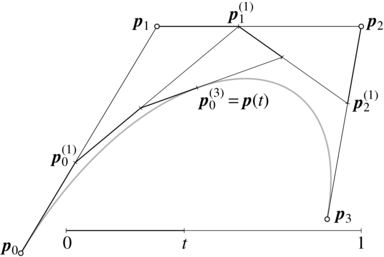
\includegraphics[scale=0.5]{decas.png}

\clearpage
\subsection*{Zadanie 6}
Zadanie nie jest wcale trudne, wystarczy wyłączać $(1-t)$. Najpierw wprowadźmy oznaczenie $s=(1-t)$ dla uproszczenia. Mamy:\\
$$P(t)=\sum\limits_{i=0}^n B_i^n(t)W_i = \sum\limits_{i=0}^n {n \choose i}t^i s^{n-i} W_i$$
$$P(t) = {n \choose 0} t^0 s^{n} W_0 + {n \choose 1} t^1 s^{n-1} W_1 + \dots + {n \choose n-1}t^{n-1} s^1 W_{n-1} + {n \choose n}t^n s^0 W_n$$
$$P(t) = \left( \dots \left( W_0 {n \choose 0} s + W_1 {n \choose 1}t\right) s + \dots + W_{n-1}{n \choose n-1}t^{n-1}\right)s + W_n{n \choose n}t^n $$
Dodatkowo, z Dyskretnej wiemy, że:
$${n \choose i} = {n \choose i-1} \cdot \frac{n+1-i}{i} $$
Algortym działający w czasie $O(n)$:\\
$s = 1-t;\\
b=n; $ - dwumian newtona\\
$p=p_0; $ - wynik\\
$d=1;$ - $t^n$ \\
for $i=1$ to $n$ do\\
\phantom{xx}$p=p\cdot s + b\cdot p_i\cdot d ;$\\
\phantom{xx}$d=d\cdot t;$\\
\phantom{xx}$b=(b\cdot(n-i))/(i+1);$\\
end\\
return $p;$


\subsection*{Zadanie 7}
Nie jestem pewien, ale (wiedząc, że, kiedy mamy sumę w liczniku i sumę w mianowniku, możemy każdy składnik sumy z licznika podzielić najpierw przez sumę z mianownika - w końcu tak działa dodawanie ułamków o tym samym mianowniku):

$$R_n(t)=\frac{\sum\limits_{i=0}^n w_iW_iB_i^n(t)}{\sum\limits_{i=0}^nw_iB_i^n(t)} = \sum\limits_{i=0}^n \frac{w_iW_iB_i^n(t)}{\sum\limits_{j=0}^nw_jB_j^n(t)} = \sum\limits_{i=0}^n \frac{w_iB_i^n(t)}{\sum\limits_{j=0}^nw_jB_j^n(t)}\cdot W_i$$
Teraz z wykładu wiemy, że $$\alpha_0 W_0  + \alpha_1 W_1 + \dots + \alpha_n W_n$$ 
jest kombinacją barycentryczną punktów (dla $W_0 \dots W_n$ - punktów $\alpha_0 \dots \alpha_n$ - liczby rzeczywiste) $\Leftrightarrow$ gdy $\sum\limits_{i=0}^n \alpha_i = 1$. 
Skoro tak, to:
$$ \frac{w_iB_i^n(t)}{\sum\limits_{i=0}^nw_iB_i^n(t)} $$
Jest naszym $\alpha_i$, więc:
$$ \sum\limits_{i=0}^n \frac{w_iB_i^n(t)}{\sum\limits_{j=0}^nw_jB_j^n(t)} = \frac{\sum\limits_{i=0}^n w_iB_i^n(t)}{\sum\limits_{i=0}^nw_iB_i^n(t)} = 1$$

A to jest to co chcieliśmy pokazać, więc $R_n(t)$ jest kombinacją barycentryczną punktów, więc można go utożsamić z punktem.
\end{document}
